\documentclass[11pt]{article}

%%\usepackage{lucbr,graphicx,fancyhdr,longtable}
\usepackage{lucidabr,graphicx,fancyhdr,longtable}

\newcommand{\kc}{\textsf{kCARTA}\xspace}
\newcommand{\cm}{\hbox{cm}}

% make a single, doubly indented line 
% (mainly used for driver file examples)
\newcommand{\ttab}{\indent\indent}

\input ASL_defs

\setlength{\textheight}{7.5in}
\setlength{\topmargin}{0.25in}
\setlength{\oddsidemargin}{.375in}
\setlength{\evensidemargin}{.375in}
\setlength{\textwidth}{5.75in}

\newlength{\colwidth}
\setlength{\colwidth}{8cm}
\newlength{\colwidthshort}
\setlength{\colwidthshort}{6cm}

\definecolor{light}{gray}{0.75}

\pagestyle{fancy}

% \date{July 5, 1994} % if you want a hardcoded date

\lhead{\textbf{\textsf{DRAFT}}}
\chead{kCARTA}
\rhead{\textsf{Version 1.10}}
\lfoot{UMBC}
\cfoot{}
\rfoot{\thepage}

\newcommand{\HRule}{\rule{\linewidth}{1mm}}
\newcommand{\HRulethin}{\rule{\linewidth}{0.5mm}}

\begin{document}
\thispagestyle{empty}
\vspace{2.0in}

\noindent\HRule
\begin{center}
\Huge \textbf{\textsf{kCARTA}}: Installation and Testing
\end{center}
\noindent\HRule

\vspace{0.75in}
\begin{center}
\begin{Large}
Sergio De Souza-Machado, L. Larrabee Strow,\\ Howard Motteler and Scott
Hannon
\end{Large}
\end{center}

\vspace{0.5in}
\begin{center}
Physics Department\\
University of Maryland Baltimore County\\Baltimore, MD 21250 USA\\
\end{center}

\vspace{0.5in}
\begin{center}
Copyright 2000 \\
University of Maryland Baltimore County \\
All Rights Reserved\\
v1.10  \today\\
\end{center}

\vfill

\noindent\HRulethin
\begin{flushleft}
\begin{tabbing}
Sergio~De~Souza-Machado: \=    sergio@umbc.edu \\
L.~Larrabee~Strow:   \>        strow@umbc.edu\\
\end{tabbing}
\end{flushleft}

%\begin{flushright}
%\includegraphics[width=1.0in]{umseal.eps}
%\end{flushright}

\newpage
\tableofcontents
\listoftables
\listoffigures
\newpage

\begin{center}
{\bf ABSTRACT}
\end{center}
\kc is a radiative transfer code for a scattering or non-scattering Earth's
atmosphere.  It can be used to output monochromatic gas optical
depths, layer-to-space transmittances and radiances.  The basic version can 
perform clear sky radiative transfer and jacobian computations, while the
advanced version can perform scattering computations. The user can easily 
change satellite viewing angles and surface boundary conditions, and/or insert 
clouds or aerosols. 

\kc v1.09+ allows the user to arbitrarily set the atmosphere layering 
structure. The namelist files required to steer a run are easy to create.  We 
hope that the ease of use, range of features and speed of \kc, make it a 
useful tool.

In addition to the main \kc source code, we provide many packages that need 
to be picked up so that this code can be run. One is $klayers$, which allows 
an user to input a radiosonde or retrieved point profile, and output a layer 
averaged profile that \kc can use. Another is $RTP$ which is the file format
that the AIRS Level II products will be saved in.

We also provide some simple scripts to take a radiosonde profile and convert 
it to a layer averaged RTP profile, as well as another script that runs an
input namelist file through \kc and produces the specified output. Fortran and
Matlab source code that enables on to read the output from \kc is also 
supplied.

\newpage
\section{Introduction}

\kc stands for ``kCompressed Atmospheric Radiative Transfer
Algorithm.''  This is an infrared, ``monochromatic'' radiative
transfer algorithm written for a one dimensional non-scattering Earth
atmosphere.  The program can either assume a plane parallel
atmosphere, or include effects on the satellite viewing angle due to
the curvature of the earth. In addition, the code can compute the radiances 
for either an uplooking or a downlooking instrument. 

\kc is driven by a namelist file. This file sets run time parameters, such as
wavenumber bounds, and atmospheric boundary conditions. In addition, \kc 
expects a layer averaged profile. We supply a code, $klayers.x$ that takes a 
point profile, and outputs a layer averaged profile.

Many users will want to quickly compute optical depths, or layer to space 
transmittances, as well as clear sky radiances. This document explains helps 
the user set up the basic excutable version of \kc, and explains many 
examples.  Refer to the complete documentation for more information, as well 
as using some of the more advanced features of \kc

\section{Installing and compiling \kc}
This is for the user that wants to install and use \kc as quicly as 
possible. First the user has to obtain the software and the kCompressed
database files. We assume at this point that the user reads and familiarises
him//herself with the $README.1ST$ file that is in the main directory. Many of
the points raised and discussed in that file are repeated here. 

The files then need to be installed, after which the code has to be compiled. 
Finally the code can be tested by running some scripts.

\section{The \kc distribution}
The distribution is divided into four parts :
\begin{itemize}
\item \textcolor{blue} {Main tarfile $kcartaYYY.tar$} where $YYY$ is the 
version number. This will contain the source code distribution (which includes
the radiative transfer code \kc and some Matlab and Fortan readers). There are
also some scripts, test files and the documentation. This is about 20Mb\\
\item \textcolor{blue} {Bugfix tarfile $kcarta\_bugfixYYY.tar$} where $YYY$ 
is the version number. This will contain the bugfixes, mainly to the 
\kc source code. This tar file is about 3Mb. Both the above tar files can
be obtained from our ftp site.\\
\item \textcolor{blue} {kCompressed Database} : about 600Mb, supplied on 
CDs. We supply two versions, the big endian or the little endian versions. 
This compressed database was computed using our custom line-by-line code, 
which allows us to fine-tune the lineshapes (eg line mixing for CO2)\\
\item \textcolor{blue} {supplementary data tarfile kcartaDATA.tar} : This 
contains the text and datafiles necessary to run \kc, such as the reference
profiles for each of the HITRAN gases, the solar intensity at TOA, CKD water
continuum and so on. This tarfile is about 35Mb\\
\end{itemize}

In addition, the user needs to obtain the following two packages
\begin{itemize}
\item \textcolor{blue} {RTP} : Contains the source code that is necessary
to read and use RTP files. This package is absolutely necessary, as it is
the file format in which the layer averaged profiles are read in by \kc \\
\item \textcolor{blue} {KLAYERS} : Contains the source code that takes in a
user supplied point profile and outputs a (100 AIRS) layers averaged profile.
The input file should be an RTP file, and the output file would also be RTP.\\
Typical usage : \\
   klayers\_airs fin='level.prof.in.rtp' fout='layers.prof.out.rtp' nwant='-1'
\item \textcolor{blue} {SARTA} : If the user also wants to utilise the AIRS
Fast Forward Model that was developed at UMBC, using \kc, then this package
needs to be picked up and used as well.\\
Typical usage : sarta\_nom fin='layers.prof.out.rtp' fout='answers.out.rtp'
\end{itemize}

\subsection{Installing \kc}
Having obtained all the above six packages and databases, the user can 
start to install \kc :
\begin{itemize}
\item \textcolor{blue} {Untar $kcartaYYY.tar$} :  this will create a main 
subdirectory, named \kc, as well as many subdirectories containing the 
source code, scripts, utility code and so on.
\item \textcolor{blue} {Untar $kcarta\_bugfixYYY.tar$} :  This will 
overwrite the relevant source code files with the latest ones that are 
deemed bugfree. 
\item \textcolor{blue} {Install datafiles} : Under the KCARTADATA 
subdirectory, the user can install the basic data files that are required at
run or compile time (such as reference database profile, solar radiance at 
TOA etc).
\item \textcolor{blue} {Install databasefiles} : Under the KCARTADATA
subdirectory, the user can install (or provide symbolic links to) the 
$CompDataBase$ and $WaterDataBase$ files provided in the diskettes 
containing the kCompressed Database. Or the user can set up these files in
any directory he/she pleases
\item \textcolor{blue} {Create a WORK directory} : Create directory WORK
under the KCARTA directory, if it does not exist.
\end{itemize}

Below is an example of the data file set up that we at UMBC use for our Linux 
machines. Note that this set up corresponds $EXACTLY$ to that specified in the
$kcarta.param$ parameter file
\begin{verbatim}
paths/directories eg on our local system here at UMBC, the 
1) database is at 
      PARAMETER (kWaterPath  = '/asl/data/kcarta/v20.ieee-le/h2o.ieee-le/')
      PARAMETER (kCO2Path    = '/asl/data/kcarta/v20.ieee-le/etc.ieee-le/')
      PARAMETER (kCompPath   = '/asl/data/kcarta/v20.ieee-le/etc.ieee-le/')
2)continuum, solar and cross-section data is at
      PARAMETER (kCKDPath    = 
     $              '/asl/data/kcarta/KCARTADATA/General/CKDieee_le/')
      PARAMETER (kSolarPath = 
     $              '/asl/data/kcarta/KCARTADATA/General/SOLARieee_le/')
      PARAMETER (kXsecFile  = 
     $              '/asl/data/kcarta/KCARTADATA/General/xsecdata.dat.intel')
3)database listing files compHT1998.param and xsecHT1998.param are at
      PARAMETER (kXsecParamFile = 
     $              '/asl/data/kcarta/KCARTADATA/General/xsecHT1998.param')
      PARAMETER (kCompParamFile = 
     $              '/asl/data/kcarta/KCARTADATA/General/compHT1998.param')

\end{verbatim}

A diagram describing how $RTP$, $KLAYERS$, $SARTA$ and $KCARTA$ interact with
each other, is shown below.
\begin{figure}
\includegraphics[width=5.5in]{FIG/interact.eps}
\caption{Interaction of our various packages : $RTP, KLAYERS, SARTA, KCARTA$}
\end{figure}

\section{Directory structure}

The directory/subdirectories contain the k-compressed code, tests
and so on.  Many of the subdirectories have additional ``readme''
files, describing further what is contained in the files. A brief
synopsis of each subdirectory follows.

\begin{verbatim}

 BIN      home for executables
          After you type ``make'' in either SRC or UTILITY, successful 
          compilation in either subdir will put the executables here

 DOC      somewhat detailed documentation

 INCLUDE  parameter include files
          You need to edit these files to tell kCARTA where to find very
          important files at run time, and how large to set its arrays
          at compile time

 LIB      blas libraries
          We are having wierd problems with the Linux supplied libraries
          (uppercase vs lowercase). So we recommend compiling our 
          LIB/blas.ref package with the uppercase option (as supplied), and
          linking to it and the LU77 library

 MATLAB   sample matlab v5.0+ code to read and plot kCARTA output
          So much easier and convenient than the f77 readers

 SCATTERCODE
          If you want to do scattering computations, this subdirectory will
          let you generate MIE parameter files (using Frank Evans code)

 SCRIPTS  demonstration shell scripts
          comp.sc       figures out what compressed database files you have
                        and puts results in blah/xsecHT1998.param,
                        blah/compHT1998.param
                        You might need to edit this file as necessary, since 
                        you need to set the same paths to these two files as 
                        are are parameters kXsecParamFile,kCompParamFile in 
                        INCLUDE/kcarta.param
          makeprof_TXT2RTP.sc 
                        takes in a specified TEXT point profile, and runs it
                        through makeRTP.x (to change it to a RTP format). The
                        resulting file is then run through klayers, and 
                        now this final resulting RTP file can be used as a
                        layer averaged profile for KCARTA
                        Usage : basic.sc inTEXTprofile outRTPfile
          makeprof_RTP2RTP.sc 
                        takes in a specified RTP point profile, and runs it
                        through klayers. This resulting RTP file can be used 
                        as a layer averaged profile for KCARTA
                        Usage : basic.sc inRTPprofile outRTPfile
          basic110_TXT2BIN.sc      
                        takes a user specified .nml (namelist) file and 
                        produces a KCARTA output file. It assumes that the
                        point profile is in a TEXT format
                        Usage : basic.sc inNameListFile outkcfile
          basic110_RTP2BIN.sc      
                        takes a user specified .nml (namelist) file and 
                        produces a KCARTA output file. It assumes that the
                        point profile is in a RTP format
                        Usage : basic.sc inNameListFile outkcfile
          kcwrap        Our end-all super-dooper script
                        Takes in a RTP level profile, chugs it thru KLAYERS,
                        then thru KCARTA, and then does an AIRS convolution!
                        Assumes you have MATLAB, and that you have correctly
                        specified the atmospheric parameters in the driver
                        RTP file (ie KCARTA assumes kRTP = +1). Also assumes
                        you have a whole bunch of RTP tools and AIRS SRF files
                        that have been written by our ASL group at UMBC

 SRC      source code 
          The kCARTA source code is here .. database uncompression, clear
          sky radiative transfer and jacobians, scattering using RTSPEC,
          DISORT and kTWOSTREAM. The Makefile produces :
          make, make basic : produces ../BIN/bkcarta.x == basic kCARTA version
          make scat        : produces ../BIN/kcarta.x  == scattering kCARTA 

 TEST     files and directories to see if your installation of KCARTA worked.
          You might need to edit test.sc and diffemeall.sc to get the 
          subdirectories correctly set up
          test.sc        runs one profile thru ../BIN/bkcarta.x for a series 
                         of small frequency intervals.
          diffemall.sc   reads in the output produced by running test.sc and
                         compares the results to files we supply. Modulo small
                         errors in number representation, there should be no
                         differences betweene what you get and what we supply!

 UTILITY  various utility programs 
          If your fseek works fine, great! (use g77)
          If not, you need to use the slower READwoFSEEK readers
          The Makefile in this directory produces the following executables
          in the ../BIN directory : 
          readkcarta.x    this reads the output versions of KCARTA that include
                          summaries of input namelist friver file and profile
          readkcBasic.x   this reads simplest basic output version of KCARTA
          readjacob.x     this reads the jacobian output of KCARTA
          readflux.x      this reads the flux output of KCARTA
          makeRTPfile.x   this takes in a text point profile and outputs
                          an RTP point profile
          compdatabase.x  this will fly thru your compressed database files
                          and produce a summary of which files you do have. 
                          This list is needed by KCARTA at run time.

 WORK     your KCARTA testing and running is done here
          This directory does not come with the TAR package, so to prove you 
          read this file, you need to make this subdir. Else when you go to 
          the  TEST directory and type ``test.sc'' things will go awry.


\end{verbatim}

\section{Compiling the \kc source code}
Now the source code compilation can begin. There are three main sets of code
that have to be compiled. We will decribe the compilation assuming the user 
is going to use the 100 AIRS pressure layers/levels, instead of changing the 
pressure levels. Before compiling each of the three packages described below, 
the user should edit the relevant Makefile so that his/her preferred F77 
compiler will be called. We have tested the package mainly on Unix style 
SGI and Absoft machines. The flags for these compilers are
\begin{verbatim}
# SGI Fortran
# ------------
# SGI compiler options
# -u  : turn off implicit typing of variables
# -g  : generate debugging information (turns off optimization)
# -C  : do run time subscript range checking
# -w0 : inform about unused variables 
# -O3 : heavy optimization
# -64 : 64-bit objects (libraries must match)
#
#F77=/usr/bin/f77
## FLAGS = -static -C -col120
#FLAGS = -static -O2 -64 -col120 -C
#UFLAG = -u
#LIBS  = -lblas -lcomplib.sgimath
#FDOUBLE = -r8

# Linux with Absoft Fortran
# --------------------------
# Absoft compiler options
# -f    fold all names to lower case
# -N109 fold all names to upper case
# -W    wide source file
# -w    suppress warning messages (absoft is more fussy than SGI or g77)
# -A    alignment warnings
# -C    check array bounds
# -O    some optimizations
# -N3   add record info to unformatted files
# -s    static allocation
# -N2   force intrinsic double functions
# -N113 force double precision 
# -N114 force untyped variables as warnings
# -g    symbol and line info included, for debugging purposes
F77=f77
# FLAGS = -w -W -C -N3 -s -N109
UFLAG = -N114
FLAGS = -w -W -O -C -N3 -s -N109
FLAGS_RTP = -w -W -O -N3 -s
LIBS = -lU77 -L ../LIB/blas.ref -lblas 
FDOUBLE = -N2 -N113
\end{verbatim}

If Absoft is used, there might be a few warning messages produced during the 
compilations as it is quite fussy.

\begin{itemize}
\item \textcolor{blue} {RTP} Go to RTP/Src and edit the ``Makefile'' so that 
the compiler options are those that exist on your machine, and the HDF
paths point to valid HDF paths on your computer. Type ``make''. This
should produce a library file \textcolor{red}{librtp.a}.
\item \textcolor{blue} {klayers} Go to KLAYERS/Src and edit the 
``Makefile'' so that the compiler options are those that exist on your 
machine, and the HDF and RTP libary packages point to valid addresses. 
Type ``make''. This should produce a file \textcolor{red}{klayers.x}.\\
To check that this executable file works, go to KCARTA/SCRIPTS and type 
\textcolor{red} {makeprof.sc BASIC/USStandardProf\_NEW WORK/test.op.rtp}
If everything is OK, a file named ``test.op.rtp'' should appear in the WORK
subdirectory. If things do not work, you might have to edit the makeprof.sc
file so that the path names are valid
\item \textcolor{blue} {SRC symbolic link} :  At the main KCARTA 
subdirectory, make sure that the ``SRC'' symbolic link points to ``SRCv1.10''
\item \textcolor{blue} {BLAS library} : If your computer has a BLAS library, 
you can skip this part. Else go to KCARTA/LIB/blas.ref subdirectory, and 
type ``make'' (at present the Makefile assumes a LINUX Absoft F77 compiler.
Actually if funny things happen at link time, it might behoove you to use this
library, as there seem to be some unresolved issues about uppercase vs 
lowercase (notice most of our compiler options turn everything to uppercase).
\end{itemize}

Now you need to edit the $INCLUDE/kcarta.param$ file.You need to ensure that 
the kCompPath, kCPO2Path and kWaterPath strings point correctly to the 
database files, while kCKDPath, kSolarPath and kXsecFile point to the correct 
be vs le files. In addition you need to set the sizes of the arrays.

Now you need to set up the KCARTA/SRCv1.10/Makefile so that the compiler 
options are those that exist on your machine.  You also need to ensure that 
the HDF and RTP paths point to the correct directories where these libraries 
exist. 

You are now ready to compile \kc. The \kc Makefile can make any one of two 
different executables. For the basic distribution, simply typing ``make'' will
produce \textcolor{red} {bkcarta.x} in the KCARTA/BIN directory. This basic
version of \kc can do mixed path, radiances and jacobian computations.

A more ambitious user might want to compile the scarttering versions of \kc.
This can be done by editing the Makefile as necessary. This increases the 
complexity and memory usage, but enables you to obtain all the all the 
features of the basic kCARTA package (optical depths, clear  sky radiative 
transfer, clear sky jacobians and fluxes), as well as $kTWOSTREAM$, $DISORT$ 
and $RTSPEC$ scattering radiances and fluxes. However, this version uses a 
$LOT$ of memory

\section{Compiling the \kc utility source code}
You now need to compile the f77 readers and utility files. Go to 
KCARTA/UTILITY.

\begin{itemize}
\item \textcolor{blue} {readers with fseek}  If your compiler supports the  
``fseek'' subroutine, type ``make'' at the prompt. If everything compiles ok, 
file \textcolor{red}{readkcBasic.x} will appear in the KCARTA/BIN directory.
Note that Absoft F77 actss funny with the fseeks, so the default compiling 
for LINUX machines is to use $g77$. If your compiler happily uses fseeks , you
might need to edit files $readkcBasic.f$ and $readbinary.f$, replacing 
\textcolor{red}{iDummy = fseek(,...)} with
\textcolor{red}{CALL fseek(,...)} with
as well as removing FSEEK from the local variables declarations
\item \textcolor{blue} {readers without fseek} Go to 
KCARTA/UTILITY/READwoFSEEK. If your compiler does not support the 
``fseek'' subroutine, type ``make'' at the prompt. If everything compiles ok, 
file \textcolor{red}{readkcBasic.x} will appear in the KCARTA/BIN directory.
\end{itemize}

\section{How to check the \kc installation, using script basic.sc}

If all this has been accomplished successfully, the user is now ready to try 
running \kc. Change to the KCARTA/SCRIPTs directory and type \\
\begin{center}
\textcolor{red} {basic.sc sondeprofile outputfile}
\end{center}

Here $sondeprofile$ is the name of the input radiosonde profile. 
This input profile will be processed through $klayers.x$, producing a layer
averaged profile $klayers.op.rtp$ in the KCARTA/WORK subdirectory. After that,
$bkcarta.x$ runs, reading in namelist file $basic.nml$ (see below) and profile
$klayers.op.rtp$. The output of \kc is stored in a large binary file,
$outputfile$.  This binary output file consists of a header, which
contains information that determine the overall size of the file. After this 
comes the actual binary data. Since \kc works in chunks of 10000 points, 
all the outputs for the first 10000 points are written out, followed by the
outputs for the next 10000 points and so on. 

As an example to use this script, type 
\begin{center}
basic.sc BASIC/USStandardProf\_NEW ../WORK/out.dat
\end{center}

To read the contents of this file, one can use either the $readkcBasic.x$ 
(Fortran) or the $readkcBasic.m$ (Matlab) readers. These readers go ahead 
and ``unchunk'' the data, as shown in the figure below. 

As would be evident from reading the more extensive documentation, \kc works 
in chunks of 10000 points. For example, suppose the user wants 100 mixed 
paths to be output from 605 to 705 $cm^{-1}$ . These mixed paths, 1-100, in 
region 605-630 $cm^{-1}$ are processed and output first. These are followed 
by the 100 mixeed paths in region 630-655 $cm^{-1}$, and so on.

However, most users would want the data in the following format. Mixed path 
1, from 605 to 705 $cm^{-1}$, followed by mixed path 2 in this complete 
wavenumber interval, and so on, uptil mixed path 100. As seen from the 
diagram, the  $readkcBasic.x$ (Fortran) and the $readkcBasic.m$ (Matlab) 
readers ``reshape'' the matrices that \kc outputs, to be in this more
convenient format.

$basic.sc$ calls $readkcBasic.x$ and translates file $../WORK/out.dat$ 
(on the left) to a very simple binary file $../WORK/outfile.bin$ 
(on the right of the figure). The only possible problem is that to make this
Fortan reader work fast, we have used the nonstandard ``fseek'' option. 
This seems to work fine with SGI Fortran and PDF77,g77 on Linux, but causes 
grief if used with Absoft.

\begin{figure}
\includegraphics[width=5.5in]{FIG/example_109.eps}
\caption{Translating the output file.}
\end{figure}

The format of the final binary file (shown on the right in the figure above)
is very simple :
\begin{itemize}
\item iSetMin : 1 integer, stating starting index (= 1)
\item iSetMax : 1 integer, stating ending index (= 10000 x iNumChunks)
\item iTotal  : 1 integer, telling how many outputs per chunk
\item Freqs   : 10000 x iNumChunks, giving the kCARTA wavenumbers (reals)
\item Data    : (10000 x iNumChunks) x iTotal, giving the data (reals)
\end{itemize}
If  $ 10000 x iNumChunks = iX$ then the $Freqs$ are output in one Fortran
data block. Similarly the $Data$ is in iTotal rows, each of which contain 
$iX$  elements. So the whole file can be read using a simple program such as

\begin{verbatim}

integer iOUN,iSetMin,iSetMax,iTotal,iX,iR,iFr,iRows,iChunks
real raWaves(10000*iChunks),raaData(iRows,10000*iChunks)

read(IOUN) iSetMin
read(IOUN) iSetMax
read(IOUN) iTotal
iX = iSetMax - iSetMin + 1
read(IOUN) (raWaves(iFr),iFr = 1,iX)
DO iR = 1,iTotal 
  read(IOUN) (raaData(iR,iFr),iFr = 1,iX) 
  END DO 
\end{verbatim}
Typically, for a 100 layer atmosphere, iTotal is about 500 (five sets of 
mixed paths), while iX is an integer multiple of 10000 points (eg for a 
typical AIRS channel, this would probably span one or two kCARTA chunks, which
would be about 10000 or 20000 points).

\section{Units and Definitions}

All angles set in the \kc files should be in degrees.
Frequencies are in units of wavenumbers (\wn).  In defining the
atmospheres inside the $nm\_radnce$ section, pressure boundaries should be
in millibars (1.0 atm=1013.25 mb).  Surface and deep space temperatures
are in Kelvin.  If the user specifies pressures at which radiances are
to be output, they should also be in millibars.

The gas profiles expected by \kc use the following units.  The gas
amounts are path averaged over the layers, and are in units of
$\hbox{\em kiloMoles} \cm^{-2}$.  Temperatures should be
specified in {\em kelvin}, while pressures and partial pressures
should be expressed in {\em atmospheres}.  Layer altitude
(approximately at center of the layer) should be in {\em
kilometers}.  Each gas will have a kProfLayer layer profile.  Note that if
the user inputs a point profile in the appropriate format to our
supplied {\sf kLayers} program, the path averaged profile that is
output by this program will be in the correct units.

Output gas and mixed path optical depths are dimensionless (absorption
coefficient $\times$ gas amount); obviously so are transmittances.
Output radiances are in blackbody radiance units ($\hbox{\em watts}
\;\ m^{-2} sr^{-1}/\cm^{-1}$).  

\section{KCARTA Readers and Miscellaneous files}

The output produced by successful runs of \kc can be read using our supplied
Matlab of F77 readers. Note as mentioned above, Absoft F77 does not seem to
like the fseek routines, so LINUX users could use g77 to compile the reader 
code.

\subsection{Files in MATLAB subdirectory}

The most useful files are

\begin{description}

\item[readkcstd.m:] standard reader, for the binary output file from
  kcarta.x. Allows user to save all spectra.

\item[readkcjac.m:] reads in the jacobian binary output file from
  kcarta.x.  

\item[readkcflux.m:] reads in the flux binary output file from
  kcarta.x.  

\item[readkcBasic.m:] reads in the very simple binary output file from
  kcarta.x.  

\end{description}

\subsection{Files in UTILITY subdirectory}

The supplied Makefile compiles these files and stores the
executables in the BIN subdirectory

\begin{description}

\item[readkcarta.f:] standard reader, for the binary output file from
  kcarta.x. Allows user to save all spectra.

\item[readjacob.f:] reads in the jacobian binary output file from
  kcarta.x.  

\item[readflux.f:] reads in the flux binary output file from
  kcarta.x.  

\item[readkcBasic.f:] reads in the very simple binary output file from
  kcarta.x.  

\item[compdatabase.f:] is used to create the parameter files comp.param 
 and xsec.param (which get renamed to compNN.param, xsecNN.param); these two
 files list the compressed files in the database. $NN$ helps tell you which
 is the database version you are using. For example, H1996  means 
 ``built with HITRAN 1996'', H1998  means ``built with HITRAN 1998'', 
 and HT1998 means ``built with HITRAN 1998 + Toth''

\item[makeRTPfile.f:] is used to take in a test point profile and write out
 a RTP point profile that can be run throught $klayers.x$.
\end{description}

\section{Files in SCRIPTS subdirectory}

\begin{description}

\item[comp.sc:] is a script file that uses compdatabase.x to go
  through the available k-compressed files in DATA/CompDataBase and
  DATA/WaterDataBase, eventually storing the summary result in
  SRC/comp.param, which is a file needed by kcarta.x.  To make this
  script executable, type ``chmod +x comp.sc'' at the UNIX prompt.
  Each time you add/remove files from the compressed database, this
  script should be run to update comp.param (which gets renamed to 
  blah/compHT1998.param, blah/xsecHT1998.param) and thus let 
  kcarta.x run merrily.

\item[basic.sc:] is a script file that allows user to input a radiosonde
  profile name and a kcarta output name. This script then calls the 
  klayers.x program, the bkcarta.x program and the readkcBasic.x program. 
  This has already been described above.

\item[makeprof.sc:] is a script file that allows user to input a radiosonde
  profile name and output a KLAYERS layer profile in  RTP format.

\item[kcwrap:] is thge big-daddy script file. This allows user to take an 
  input levels profile (in RTP format), check to ensure that it contains all
  necessary atmospheric info to drive a KCARTA run. Having done this, the
  chosen levels profile from the RTP file is output to another RTP file (along
  with the wavenumber bounds and atmospher info), and is run thru $KLAYERS$.
  Since this generates a AIRS 100 layer profile, $KCARTA$ can now be run.
  After this, the $KCARTA$ output is convolved with the AIRS SRFs, and the
  results are stored in an RTP file. This is an awesome template for people
  to mess around with ... obviously, with some modifications of the driver
  namelist template, $KCARTA$ can be used to output mixed paths, jacobians 
  and so on; these can be convolved as appropriate, to perform sensitivity
  studies or make Fast Models etc .....

\end{description}

If the user is still living in the era of $kCARTA$ $v1.09-$, he/she will not 
be using RTP profiles and so needs a $text$ levels profile to send through 
$KLAYERS$. As distributed, $basic.sc$ is symbolically linked to 
$basic110\_TXT2BIN.sc$; this contains an intermediate step where the input
text levels profile is translated to a RTP levels file, as this is the only
format supported by $KLAYERS$. (Essentially, $makeprof\_TXT2RTP.sc$ takes in
a text level profile, converts it to a RTP level profile, and then runs this
through $KLAYERS$).

\begin{figure}
\includegraphics[width=5.5in]{FIG/txt2bin.eps}
\caption{Taking a text level profile and producing $KCARTA$ binary output.}
\end{figure}

If the user is living in the era of $kCARTA$ $v1.10+$, he/she will probably 
be using RTP files, and so the user can symbolically link $basic.sc$ to 
$basic110\_RTP2BIN.sc$. (Essentially, $makeprof\_RTP2RTP.sc$ takes in a RTP
level profile, and then runs this through $KLAYERS$).

\begin{figure}
\includegraphics[width=5.5in]{FIG/rtp2bin.eps}
\caption{Taking a RTP level profile and producing $KCARTA$ binary output.}
\end{figure}

$comp.sc$ goes through the database files that you have, eventually producing
files $xsecHT1998.param$ and $compHT1998.param$. These two files are needed by
$KCARTA$ at run time, as it enables it to decide whether the spectroscopy 
database files for a given gas, in a given wavenumber interval, do exist or
not. Parameters $kXsecParamFile, (kCompParamFile$ must be set to correctly
point to the files produced by running $comp.sc$

\begin{figure}
\includegraphics[width=5.5in]{FIG/comp.eps}
\caption{Checking the distributed database.}
\end{figure}

$kcwrap$ is the mother of all scripts. The user can use it to take an input
RTP level profile, and produce a convolved $KCARTA$ output (convolved with the
AIRS srfs). The savvy user can modify the script to produce eg fast models, 
or convolutions with other instruments.

\begin{figure}
\includegraphics[width=5.5in]{FIG/kcwrap.eps}
\caption{kcwrap - the ultimate wrapper.}
\end{figure}

\section{Additional Testing and More Information}

Having quickly installed and set up \kc, the user can now further read this
document and perform further tests to see if the set up produces results that
agrre (within roundoff error) to those in our supplied comparison files. 
Go to the KCARTA/TEST subdirectory and type ``test.sc''. This will run a 
profile throught $klayers.x$, after which \kc is used to compute TOA radiances
for a set of specified wavenumber intervals. Having doe this, type 
``diffemall.sc'' ... this will compare your results to the ones we supply. 
Within roundoff error, they should be the same!

\begin{description}
\item[test.sc:] is a script file that ran various programs,
  including kcarta.x to create the data in ../COMPARISON.  To be
  able to run this script, you may need to type ``chmod +x
  kcarta.sc'' at the UNIX prompt

\item[diffemall.sc:] is a script file that runs the data files in OUTPUT
  thru our ../BIN/readkcarta.x reader, saving the output as text files.
  These text files are then individually diff'ed against the text files
  in COMPARISON, so the user can see if things worked as expected (there
  might be slight roundoff errors in the radiances).
\end{description}

\begin{figure}
\includegraphics[width=5.5in]{FIG/tester.eps}
\caption{Flowdiagram describing $test.sc$.}
\end{figure}

\subsection{Files in TEST subdirectory}

Six frequency ranges were used for testing purposes, as follows

\medskip
\begin{tabular}{cccc}
iFreqIndex = 1 &      r1= 755.0 & to &   r2=780.0 \\
iFreqIndex = 2 &      r1=1005.0 & to &   r2=1055.0\\
iFreqIndex = 3 &      r1=1230.0 & to &   r2=1255.0\\
iFreqIndex = 4 &      r1=1430.0 & to &   r2=1505.0\\
iFreqIndex = 5 &      r1=1530.0 & to &   r2=1605.0\\
iFreqIndex = 6 &      r1=2355.0 & to &   r2=2405.0\\
\end{tabular}

\bigskip
From SCRIPTS/basic.sc and SCRIPTS/makeprofile.sc, followed by a run of
kcarta.x, some examples of the file names are

\begin{description}
\item[testprof1:]   profiles for 36 gases, using test profile 1
\item[testa1.ip:]   genln2 input file that uses profile 1,freqrange 1
\item[testa1.dat:]  resultant kcarta.x binary output file
\item[testprof14:]  profiles for 36 gases, using test profile 14
\item[teste14.ip:]  genln2 input file that uses profile 14,freqrange 5
\item[teste14.dat:] resultant kcarta.x binary output file
\end{description}

\section{The template namelist files for the tests}

For the kcarta.sc test run, one atmosphere is built up for a downward
looking instrument. The effects of background thermal radiation as well as
effects of solar radiation, are both turned off. Water continuum CKDv2.1 
is used. The atmosphere is defined between the maximum and minimum AIRS 
pressure levels. The surface emissivity is found in emissivity.dat, while 
the surface temperature is the temperature of the lowest layer (set by 
basic.sc). The template nml file is 
found under\\
\begin{verbatim}
../DATA/TemplateNML/kcartainput_template.nml
\end{verbatim}

See kcarta1.10.ps for examples and more detailed information on the
format of driver files.

\section{Example template files}
This section includes a bunch of template files, which are explained in some
detail by comments inside the files. To understand these namelist files, 
please refer to the more complete documentation ($kcarta1.10.ps$ or 
$bkcarta1.10.ps$)

\subsection{basic.nml example}
This is the template file used in the $basic.sc$ script. It assumes that the
$kcarta.param$ file declares enough memeory for 6 sets of mixed paths. Five
of these are used to output optical depths for Fast Forward Model, while the
sixth set is used to compute a radiance

\begin{verbatim}
 !!!!!!this is a namelist template file to make Forward Models
 $nm_params
 namecomment    =  '******* PARAMS section *******'
 !output data in shortest easy form
 kLongOrShort = 0             
 !use water continuum CKDv2.4
 kCKD         = 24
 !compute surface temperature by interpolating layer temperatures across
 !presure levels
 kSurfTemp    = +1.0
 $end

 $nm_frqncy
 namecomment    =  '******* FRQNCY section *******'
 !start, stop wavenumbers
 rf1            = 930.0
 rf2            = 980.0

 $end

 $nm_molgas
 namecomment    =  '******* MOLGAS section *******'
 !compute optical depths of all kcomp gases + continuum
 iNGas     =            -1
 $end

 $nm_xscgas
 namecomment    =  '******* XSCGAS section *******'
 !compute optical depths of all xsec gases
 iNxsec =            -1
 $end

 $nm_prfile
 namecomment    =  '******* PRFILE section *******'
 !name of profile
 caPfname       =  'basic.prof'
 $end

 $nm_weight
 namecomment    =  '******* WEIGHT section *******'
 !this is to develop fast forward models
 !recall gases 101, 102 are the water continnum (self, foreign), which are
 !modelled sperately

 !define 6 sets of mixed paths
 iNpmix =             6
 caaMixFileLines        = 
    !all gases except water, ozone and self/for continuum have weight 1.0 (F)
    !this defines the fixed gases (F)
    '1   -1    1.0    4',
    '   1 0.0  3 0.0   101  0.0  102  0.0',
    !all gases except ozone and self/for continuum have weight 1.0
    !this defines the fixed + water gases (FW)
    '2   -1    1.0    3',
    '   3  0.0 101  0.0  102  0.0',
    !all gases have weight 1.0 except self/for continuum (FWO)
    !this defines the fixed + water + ozone gases (FWO)
    '3   -1    1.0    2',
    '101  0.0  102  0.0',
    !all gases except water and self/for continuum have weight 1.0 (FO)
    !this defines the fixed + ozone gases (FO)
    '4   -1    1.0    3',
    '   1  0.0 101  0.0  102  0.0',
    !all gases except self/for continuum have weight 0.0 (Continuum)
    !this defines the continuum gases (C)
    '5   -1    0.0    2',
    '   101  1.0  102  1.0',
    !all gases have weight 1.0
    !this defines the complete atmosphere
    !all gases have weight 1.0 
    '6   -1    1.0    -1',
 $end

 $nm_radnce
 namecomment    =  '******* RADNCE section *******'
 !define 1 atmosphere
 iNatm          =  1

 ! --------> no solar, fast thermal, emissivity file
 !use Mixed Path Set #6 to build atmospheres
 iaMPSetForRad(1)   =  6
 ! --------> atm is from 1013 mb --> 0 mb (gnd to toa)
 raPressStart(1)    =  1013.0
 raPressStop(1)     =  0.0000
 ! --------> temperature out yonder = 2.96 K
 raTSpace(1)        =   2.960000
 ! --------> earth surface temperature = 0.0 K + interpolated temperature
 raTSurf(1)         =  0.0
 !satellite is at nadir 
 raSatAngle(1)      =  0.0000000E+00
 raSatHeight(1)     =   1.000000
 ! ---------> turn solar OFF
 iakSolar(1)        =  -1
 rakSolarAngle(1)   =  25.0000000E+00
 rakSolarRefl(1)    =   1.0
 ! --------> turn background thermal ON
 iakThermal(1)      =   0
 rakThermalAngle(1) =  -1.000000
 iakThermalJacob(1) =   1
 ! --------> use emissivity file
 caEmissivity(1)    =   '../DATA/General/emissivity.dat'
 raSetEmissivity(1) =  -1.000000

 $end

 $nm_jacobn
 namecomment    =  '******* JACOBN section *******'
 !No jacobians
 iJacob =             0
 $end

 $nm_spectr
 namecomment    =  '******* SPECTRA section ******'
 !no outside spectra
 iNumNewGases   =             -1
 $end

 $nm_scattr
 namecomment    =  '******* SCATTR section *******'
 !no scattering
 iNclouds          =            -1
 $end


 $nm_output
 namecomment    =  '******* OUTPUT section *******'
 caComment      = ' OUTPUTS all MP, and rads of atms at TOA'

 !!!this says, output ALL mixed path spectra (output option #2)
 iaPrinter(1)   =    2
 iaGPMPAtm(1)   =    -1
 iaNp(1)        =    -1

 !!!this says, output radiance (output option #3) at ONE pressure = 0.0mb
 iaPrinter(2)   =    3
 iaGPMPAtm(2)   =    -1
 iaNp(2)        =    1
 raaOp(2,1)     =    00.0

 $end

 $nm_endinp
 namecomment    =  '******* ENDINP section *******'
 $end
\end{verbatim}

\subsection{test1.nml example}
This is similar to the above file, except that it completely turns off the
water continuum. In addition, it does not define any atmosphere, so it does not
compute any radiances

\begin{verbatim}
 $nm_params
 namecomment    =  '******* PARAMS section *******'
 !use all defaults params, except TURN OFF water continuum
 kCKD = -1
 $end

 $nm_frqncy
 namecomment    =  '******* FRQNCY section *******'
 !go from 755 to 780 cm-1
 rf1            = 755.000
 rf2            = 780.000
 $end

 $nm_molgas
 namecomment    =  '******* MOLGAS section *******'
 !use all gases in MOLGAS
 iNGas  =            -1
 $end

 $nm_xscgas
 namecomment    =  '******* XSCGAS section *******'
 !use all gases in XSCGAS
 iNxsec =             -1
 $end

 $nm_prfile
 namecomment    =  '******* PRFILE section *******'
 caPfname       =  'USStandard_DRY'
 $end

 $nm_weight
 namecomment    =  '******* WEIGHT section *******'
 !this is to develop fast forward models
 !this will NOT include continuum as kCKD = -1
 iNpmix =             4
 caaMixFileLines        = 
    !all gases except water and ozone have weight 1.0 (F)
    '1   -1    1.0    2',
    '   1 0.0  3 0.0',
    !all gases except ozone have weight 1.0 (FW)
    '2   -1    1.0    1',
    '   3  0.0', 
    !all gases have weight 1.0 (FWO)
    '3   -1    1.0    -1',
    !all gases except water have weight 1.0 (FO)
    '4   -1    1.0    1',
    '   1  0.0' 
 $end

 $nm_radnce
 namecomment    =  '******* RADNCE section *******'
 !no radiances
 iNatm          =  -1
 $end

 $nm_jacobn
 namecomment    =  '******* JACOBN section *******'
 !no jacobians
 iJacob =             0
 $end

 $nm_spectr
 namecomment    =  '******* SPECTRA section ******'
 !no external spectra
 iNumNewGases   =             -1
 $end

 $nm_scattr
 namecomment    =  '******* SCATTR section *******'
 !no scattering
 iNclouds         =             -1
 $end

 $nm_output
 namecomment    =  '******* OUTPUT section *******'
 caComment      = '  TEST1.IP : TO MAKE F,FW,FWO AND FO'
 !dump out ALL mixed paths (output option #2)
 iaPrinter      =    2
 iaGPMPAtm      =    -1
 iaNp           =    -1
 iaaOp          =    -1
 $end

 $nm_endinp
 namecomment    =  '******* ENDINP section *******'
 $end
\end{verbatim}

\subsection{test2.nml example}
This is used to compute radiances for two different atmospheres. It cannot
really be used to develop fast forward models. Beware that it only uses 13 
gases to build up the atmosphere (not all the gases)


\begin{verbatim}
 $nm_params
 namecomment    =  '******* PARAMS section *******'
 !use all default parameters .. which means, use kCKD = 2.1
 $end

 $nm_frqncy
 namecomment    =  '******* FRQNCY section *******'
 rf1            = 2380.000
 rf2            = 2405.000
 $end

 $nm_molgas
 namecomment    =  '******* MOLGAS section *******'
 !use the following 10 gases
 iNGas     =            10
 iaGasesNL = 1, 2, 3, 4, 5, 6, 7, 8, 9, 10
 $end

 $nm_xscgas
 namecomment    =  '******* XSCGAS section *******'
 !use the following three gases
 iNxsec =            3
 iaLXsecNL       = 51, 52, 53
 $end

 $nm_prfile
 namecomment    =  '******* PRFILE section *******'
 caPfname       =  'USStandard_DRY'
 $end

 $nm_weight
 namecomment    =  '******* WEIGHT section *******'
 !one set of mixed paths; each gas has a weight of 1.0 in each set
 iNpmix =             1
 caaMixFileLines        = '1   -1    1.0    -1'
 $end

 $nm_radnce
 namecomment    =  '******* RADNCE section *******'
 !define two atmospheres
 iNatm          =  2

 !from 700 to 0 mb, tSurf=253.34, no solar, fast thermal, emiss=0.5 (cloud)
 iaMPSetForRad(1)   =  1
 raPressStart(1)    =  700.0400
 raPressStop(1)     =  0.0
 raTSpace(1)        =   2.960000
 raTSurf(1)         =  253.34
 raSatAngle(1)      =  0.0000000E+00
 raSatHeight(1)     =   -1.000000
 iakSolar(1)        =  -1
 rakSolarAngle(1)   =  0.0000000E+00
 rakSolarRefl(1)    =  -1.0
 iakThermal(1)      =   0
 rakThermalAngle(1) =  -1.000000
 iakThermalJacob(1) =   1
 caEmissivity(1)    =   'unused'
 raSetEmissivity(1) =  0.5

 !from 900 to 40 mb, tSurf=273.34, no solar, fast thermal, emiss file
 iaMPSetForRad(2)   =  1
 raPressStart(2)    =  900.0000
 raPressStop(2)     =  40.0
 raTSpace(2)        =   2.960000
 raTSurf(2)         =  273.34
 raSatAngle(2)      =  0.0000000E+00
 raSatHeight(2)     =   -1.000000
 iakSolar(2)        =  -1
 rakSolarAngle(2)   =  0.0000000E+00
 rakSolarRefl(2)    =  -1.0
 iakThermal(2)      =   0
 rakThermalAngle(2) =  -1.000000
 iakThermalJacob(2) =   1
 caEmissivity(2)    =   '../DATA/General/emissivity.dat'
 raSetEmissivity(2) =  -1.000000
 $end

 $nm_jacobn
 namecomment    =  '******* JACOBN section *******'
 iJacob =             0
 $end

 $nm_spectr
 namecomment    =  '******* SPECTRA section ******'
 iNumNewGases   =             -1
 $end

 $nm_scattr
 namecomment    =  '******* SCATTR section *******'
 iNclouds         =             -1
 $end

 $nm_output
 namecomment    =  '******* OUTPUT section *******'
 !output radiance at 40 mb for each atmosphere (airplane flying there)
 caComment      = ' OUTPUTS RADIANCES AT *1* LEVEL FOR 2 DOWNLOOKING INSTR'
 iaPrinter      =    3
 iaGPMPAtm      =    -1
 iaNp           =    1
 raaOp(1)       = 40.0
 $end

 $nm_endinp
 namecomment    =  '******* ENDINP section *******'
 $end
\end{verbatim}

\section{Acknowledegement}
We wish to thank Dave Edwards for allowing us to use his {\sf GENLN2}
line-by-line code to generate our {\sf kCompressed} database, give us lots 
of advice on how to write our code, and allowing us to use some
modifications of his subroutines in our code. We also wish to thank Dave 
Tobin for his help in the CO2 line mixing spectroscopy. In addition, Dr. 
Gyula Molnar has provided a lot of useful feedback, regarding the meshing 
of kCARTA and kLAYERS. In addition, we wish to thank Istvan Laszlo of U. of 
Maryland, College Park for answering many questions regarding $DISORT$, and 
Frank Evans of U. of Colorado, Boulder CO for doing the same for $RTSPEC$.

\end{document}

% LocalWords:  param radiances gasIDs crosssection GasID CKDv FRQNCY freqs IDs
% LocalWords:  MOLGAS XSCGAS xsecdata ID's PRFILE AFGL gasID RADNCE endpts mb
% LocalWords:  travelling instr emiss dat FOV JACOBN jacobian PARAMS specfies
% LocalWords:  kLayer Sp kCKD ENDINP readkcarta millibars atm kelvin xsec
% LocalWords:  CFCs temps kcarta iG iX
